%!TEX root = ../thesis.tex

\section{Results}
\label{sec:results}

This section will cover the results of the verification process as it was described in section \ref{sec:checking}.
Our main finding was that there are 8 assumptions which in total grant that the properties as described in section \ref{sec:props} can not be violated, in other words: the MINRV8 architecture models the information flow properties introduced in this thesis, namely \smv{MEMORY_OP_INTEGRITY}, \smv{CSR_INTEGRITY} and \smv{NO_LEAK}, if and only if we assume the 8 assumptions that will be introduced in subsequent sections.

Additionally, roughly 22 bug fix patches\footnote{%
    The number of 22 bug fix patches was measured by counting the amount of patches containing the word \enquote{fix} in its description and being applied to the model file.
} and some \smv{INIT} constraints were applied to the model.
Taken together with aforementioned assumptions these patches mark a fixpoint of the verification process as depicted in figure \ref{fig:ver-process}.

\todo{Mention that counter-examples are in appendix}
This section is grouped as follows: section \ref{sec:assumptions} will introduce aforementioned assumptions and \smv{INIT} constraints.

Since only assumptions and no architectural refinements were introduced to the model, it was also tested how the model would behave when deliberate breaking points were introduced to it.
These breaking points tried to mimic known vulnerabilities to real-world architectures and will therefore also give an overview of the capabilities of the verification approach of this thesis.
The results to these tests will finally be presented in section \ref{sec:canaries}.

\todo{Motivation also was to test, whether these assumptions are too strong/model can actually capture weakpoints}

\subsection{Assumptions}

Technically, \smv{INIT} constraints and assumptions serve the same purpose: They limit the state spaces that will be searched for property violations.
Conceptually, however, these two concepts should be distinguished.

\subsubsection{Initial Constraints}

In the model, \smv{INIT} constraints are used to limit the search of the state space to \textit{valid} counter-examples only.
Validity here means, that properties are not false to begin with and that the initial state of the architecture complies with the specification.

We guarantee former aspect of validity by constraining the contents of registers to only contain confidential data when the model starts in machine-mode and to only contain malicious data when the model starts in user-mode.
Furthermore, cache and memory can only contain confidential data if the respective memory region is set to \textit{not} be readable for user-mode and can only contain malicious data if the respective memory region \textit{is} set to be writable by user-mode.
If, for example, the model would not be constrained to initially only contain confidential data in some register when in machine-mode, nuXmv could find a counter-example violating the \smv{NO_LEAK} property (\ref{itm:prop-no-leak}) where the architecture starts in user-mode and has confidential data in some register trivially violating the respective property.

The latter aspect of validity regarding the initial state of the model complying with the specification is guaranteed by two constraints.
The first is rather simple and is depicted in the following snippet:
\begin{lstlisting}[
    language=smv,
    caption={\gls{mstatus} \smv{INIT} constraint for the model}
]
    INIT MIE = 0b_1 -> MPP = 0b_0;
\end{lstlisting}
This constraint ensures that the interrupt handling mechanisms are set up correctly and is mandated by the RISC-V specification (cf. section \ref{sec:rv-priv-arch} and figure \ref{fig:interrupt-handling}).
No other \smv{INIT} constraints are required to set up the initial state of the model correctly.
The second constraint sets up caching correctly, i.e. if the cache is valid, it can only point to an address of a region that is cacheable and must match that addresses content unless the respective region is set to be write-back-cacheable.

\subsubsection{Property Assumptions}
\label{sec:assumptions}

\todo{Pick up point of introduction, i.e. distinction between INIT and other assumptions by concepts}

\begin{table}
    \centering
    \begin{tabular}{| c r | c | c | c |}
        \multicolumn{1}{r}{} & \multicolumn{1}{r}{} &
        \multicolumn{1}{l}{\tilthdr{\smv{MEMORY_OP_INTEGRITY} (\ref{itm:prop-mem-i})}} &
        \multicolumn{1}{l}{\tilthdr{\smv{CSR_INTEGRITY} (\ref{itm:prop-csr-i})}} &
        \multicolumn{1}{l}{\tilthdr{\smv{NO_LEAK} (\ref{itm:prop-no-leak})}} \\
        \hline % \cline{3-5}
        \multirow{2}{*}{Mode-boundary} & \smv{SAN_ON_CALL} & \checkmark & \checkmark & \\
        \cline{3-5}
        & \smv{CLR_ON_RET} &&& \checkmark \\
        \hline % \cline{3-5}
        \multirow{2}{*}{Memory} & \smv{NO_PUBLIC_READS} & \checkmark & \checkmark & \\
        \cline{3-5}
        & \smv{NO_PUBLIC_WRITES} &&& \checkmark \\
        \hline % \cline{3-5}
        \multirow{4}{*}{Memory privilege} & \smv{SAN_ON_CLASSIFICATION} & \checkmark & \checkmark & \\
        \cline{3-5}
        & \smv{CLR_ON_DECLASSIFICATION} &&& \checkmark \\
        \cline{3-5}
        & \smv{SAN_CACHE_ON_CLASSIFICATION} & \checkmark & \checkmark & \\
        \cline{3-5}
        & \smv{CLR_CACHE_ON_DECLASSIFICATION} &&& \checkmark \\
        \hline % \cline{3-5}
    \end{tabular}
    \caption{Assumptions Compared to Properties}
    \label{tbl:assumptions-overview}
\end{table}

The 8 assumptions that have been introduced throughout the verification process can be grouped into three categories:
\begin{itemize}
    \item Mode-boundary crossing related assumptions
    \item Memory related assumptions
    \item Memory privilege related assumptions
\end{itemize}

Find an overview of all these assumptions in table \ref{tbl:assumptions-overview}.
Each row represents one assumption and each column one property.
A check mark denotes that the respective assumption is critical for the respective property, i.e. there exists a counter-example proving the property to be false if the assumption at hand is not assumed.
Note that each of the assumptions is critical for at least one property.
This shows that \enquote{$ \text{assumptions} \Leftrightarrow \text{properties} $} as opposed to only \enquote{$ \text{assumptions} \Rightarrow \text{properties} $} since \enquote{$ \neg \text{assumptions} \Rightarrow \neg \text{properties} $}.

\paragraph{Mode-boundary crossing related assumptions}
As could be seen in table \ref{tbl:assumptions-overview}, there are two properties related to mode-boundary crossing.
The first of these is called \smv{SAN_ON_CALL} and mandates from machine-mode to not use \textit{dangerous} instructions before having cleared the registers from any untrusted data when entering machine-mode from user-mode.
Dangerous instructions here are \minrv{Load}, \minrv{Store}, \minrv{Csrrs} and \minrv{Csrrc} and directly stem from the properties \smv{MEMORY_OP_INTEGRITY} (\ref{itm:prop-mem-i}) and \smv{CSR_INTEGRITY} (\ref{itm:prop-csr-i}).
The next assumption to be introduced is called \smv{CLR_ON_RET}; it states: Whenever machine-mode hands back control to user-mode, the registers must be cleared of any confidential information.
The implementations of \smv{SAN_ON_CALL} and \smv{CLR_ON_RET} can be found in snippet \ref{snpt:san-on-call} and \ref{snpt:clr-on-ret} respectively.

\begin{figure}
    \begin{lstlisting}[
        language=smv,
        caption={Assumption \lstinline{SAN_ON_CALL}},
        label={snpt:san-on-call}
    ]
        G (!priv & X priv -> X (
            (priv -> !(op in { LOAD, STORE, CSRRS, CSRRC }))
            U (regs_integrity[0] = 0h_FF
                & regs_integrity[1] = 0h_FF
                & regs_integrity[2] = 0h_FF
                & regs_integrity[3] = 0h_FF)
        ))
    \end{lstlisting}

    \begin{lstlisting}[
        language=smv,
        caption={Assumption \smv{CLR_ON_RET}},
        label={snpt:clr-on-ret}
    ]
        G (
            priv & X !priv -> regs_conf[0] = 0h_00
                & regs_conf[1] = 0h_00
                & regs_conf[2] = 0h_00
                & regs_conf[3] = 0h_00
        )
    \end{lstlisting}
\end{figure}

Both assumptions \smv{SAN_ON_CALL} and \smv{CLR_ON_RET} are similar to each other.
Both were introduced under the label of being \textit{mode-boundary crossing related}, which means that both assumptions are about information flow tracking labels when changing privilege mode - more precisely: both are about the labels of register contents.
The relation of these two assumptions, however, also characterizes a pattern that can also be recognized for subsequent groups of assumptions.
It turned out that for every integrity related assumption, such as \smv{SAN_ON_CALL}, there was a similar confidentiality related assumption such as \smv{CLR_ON_RET}.
This can be easily seen in table \ref{tbl:assumptions-overview}.
In alternating rows, two groups of assumptions can be distinguished: those which are relevant to the properties \smv{MEMORY_OP_INTEGRITY} and \smv{CSR_INTEGRITY} and those which are relevant to the property \smv{NO_LEAK}.
Additionally it is noteworthy that these two groups of assumptions can be characterized by the way they constrain information flow.
Whereas confidentiality related assumptions always constrain flow of information going \textit{out of} machine-mode, integrity related assumptions always constrain flow of information going \textit{into} machine-mode.

\paragraph{Memory related assumptions}
Two assumptions about memory reads and writes join the ranks of these groups, namely \smv{NO_PUBLIC_READS} and \smv{NO_PUBLIC_WRITES} which are formally given in snippet \ref{snpt:no-public-reads} and \ref{snpt:no-public-writes} respectively.
These two assumptions don't express more than the title says; they require machine-mode to never read from or write to public memory.

\begin{figure}
    \begin{lstlisting}[
        language=smv,
        caption={Assumption \lstinline{NO_PUBLIC_READS}},
        label={snpt:no-public-reads}
    ]
        G (priv & op = LOAD -> (
            mem_addr < $REGION0_SIZE
                ? !pmpcfg0.write
                : !pmpcfg1.write
        ))
    \end{lstlisting}

    \begin{lstlisting}[
        language=smv,
        caption={Assumption \lstinline{NO_PUBLIC_WRITES}},
        label={snpt:no-public-writes}
    ]
        G (priv & op = STORE -> (
            mem_addr < $REGION0_SIZE
                ? !pmpcfg0.read
                : !pmpcfg1.read
        ))
    \end{lstlisting}
\end{figure}

\paragraph{Memory privilege related assumptions}
The four assumptions that have been introduced up to this point seem to cover all relevant channels of information transmission: registers and memory.
However, these are not enough to ensure that the MINRV8 architecture implements all information flow properties subject to this thesis.
Whereas the two memory related properties covered the group of actions by machine-mode where information directly is given to or taken from user-mode, it is also possible to transmit information indirectly via memory by writing it to or reading it from safe memory regions but doing so while changing the attributes of respective memory regions.
The two assumptions \smv{SANITIZE_ON_DECLASSIFICATION} and \smv{CLR_ON_DECLASSIFICATION} counter issues arising from these vectors.
The former assumption demands from machine-mode to ensure that a memory region does not contain malicious information when its set to be publicly inaccessible.
This assumption is formalized in snippet \ref{snpt:san-on-classify}.
The latter demands from machine-mode to always ensure that a memory region does not contain confidential information when its made publicly accessible.
This assumption is formalized in snippet \ref{snpt:clr-on-declassify}.

\begin{figure}
    \begin{lstlisting}[
        language=smv,
        caption={Assumption \lstinline{SAN_ON_CLASSIFICATION}},
        label={snpt:san-on-classify}
    ]
        G (pmpcfg0.write & X !pmpcfg0.write
            -> memory_integrity[0] = 0h_FF
             & memory_integrity[1] = 0h_FF)
        & G (pmpcfg1.write & X !pmpcfg1.write
            -> memory_integrity[2] = 0h_FF
             & memory_integrity[3] = 0h_FF)
    \end{lstlisting}

    \begin{lstlisting}[
        language=smv,
        caption={Assumption \lstinline{CLR_ON_DECLASSIFICATION}},
        label={snpt:clr-on-declassify}
    ]
        G (!pmpcfg0.read & X pmpcfg0.read
            -> memory_conf[0] = 0h_00
             & memory_conf[1] = 0h_00)
        & G (!pmpcfg1.read & X pmpcfg1.read
            -> memory_conf[2] = 0h_00
             & memory_conf[3] = 0h_00)
    \end{lstlisting}
\end{figure}

Yet, these two assumptions still not suffice to grant the absence of memory privilege related property counter-examples.
It turns out that only ensuring memory regions to not contain confidential/malicious words when (de-)classifying respective regions allows problematic data to remain in cache which bypasses \smv{SAN_ON_CLASSIFICATION} and \smv{CLR_ON_DECLASSIFICATION}.
This brings the need to also assume that the cache is cleared and sanitized by the architecture whenever a memory region is (de-)classified.
This is expressed in the assumptions \smv{SAN_CACHE_ON_CLASSIFICATION} and \smv{CLR_CACHE_ON_DECLASSFICATION} (cf. snippets \ref{snpt:sanc-on-classify}, \ref{snpt:clrc-on-declassify}).

\begin{figure}
    \begin{lstlisting}[
        language=smv,
        caption={Assumption \lstinline{SAN_CACHE_ON_CLASSIFICATION}},
        label={snpt:sanc-on-classify}
    ]
        G (pmpcfg0.write & X !pmpcfg0.write
                & cache.valid & cache.addr < $REGION0_SIZE
            -> cache.integrity = 0h_FF) &
        G (pmpcfg1.write & X !pmpcfg1.write
                & cache.valid & $REGION0_SIZE <= cache.addr
            -> cache.integrity = 0h_FF)
    \end{lstlisting}

    \begin{lstlisting}[
        language=smv,
        caption={Assumption \lstinline{CLR_CACHE_ON_DECLASSIFICATION}},
        label={snpt:clrc-on-declassify}
    ]
        G (!pmpcfg0.read & X pmpcfg0.read
                & cache.valid & cache.addr < $REGION0_SIZE
            -> cache.conf = 0h_00) &
        G (!pmpcfg1.read & X pmpcfg1.read
                & cache.valid & $REGION0_SIZE <= cache.addr
            -> cache.conf = 0h_00)
    \end{lstlisting}
\end{figure}

\subsection{Canaries}
\label{sec:canaries}

\todo{Introduce Intel x86 architecture}
In this section, it will be presented how the model of the MINRV8 architecture was altered in order to implement real-world attacks to the Intel x86 architecture.
By default, the MINRV8 architecture was not vulnerable to these attacks, however, making the architecture vulnerable will put the approach of this thesis to formally verify an instruction set architecture to a test.

\subsubsection{Cache Poisoning Attack on x86}

The - as it will be called here - cache poisoning attack was discovered and presented by Rafal Wojtczuk and Joanna Rutkowska in their publication \textit{Attacking SMM Memory via Intel CPU Cache Poisoning} \cite{Wojtczuk09}.
The term \enquote{SMM memory} refers to a specific region of memory that is designed to be only accessible by the mode of highest privilege in x86 architectures: System Management Mode.
This memory should be written only on start-up and then locked down for later write-accesses.
Wojtczuk and Rutkowska, however, managed to find a vulnerability to the x86 architecture which allowed them to effectively write to SMM memory without SMM privileges by marking respective memory region as write-back-cacheable.
The attack comprises the following steps and requires administrator privileges on the machine to be attacked:
\begin{enumerate}
    \item Mark SMM memory as write-back-cacheable using administrator privileges
    \item \label{itm:cache-pois-mem}
    Generate write accesses to the memory.
    Since the region is marked as write-back-cacheable, the writes will not be propagated to the memory controller which would drop these accesses but will be cached.
    \item \label{itm:cache-pois-smi}
    Trigger an System Management Interrupt to transfer control to System Management Mode.
    Depending on the specific addresses written System Management Mode will now execute code written with administrator privileges in step \ref{itm:cache-pois-mem}.
\end{enumerate}

Steps \ref{itm:cache-pois-mem} and \ref{itm:cache-pois-smi} can also be swapped to read from SMM memory.
Then, SMM memory will first read by SMM mode executing the interrupt handler which will leave result in some parts of the handler being cached.
After SMM returned from handling the interrupt, administrator mode can read these words from cache.

This attack does not fully apply to the MINRV8 architecture since it does not support as fine grained privilege modes as the x86 architecture.
However, the basic idea can still be implemented by following changes to the model:
\begin{itemize}
    \item For all cache transition relations, do not check whether current privilege mode suffices for the memory operation at hand, i.e. user-mode can write to cache of memory regions not set as writable to it.
    \item For load accesses to memory, do not check whether current privilege mode suffices for the memory read if the address is being cached, i.e. user-mode can read cached memory regions even if they're not set as readable to it.
\end{itemize}

These changes manage to introduce a vulnerability to the MINRV8 architecture.
If assuming all assumptions introduced in section \ref{sec:assumptions}, nuXmv manages to find a counter-example for all three information flow properties.
These are depicted in table \ref{tbl:cex-cache-vuln}.
As usual, the traces for \smv{MEMORY_OP_INTEGRITY} (\ref{itm:prop-mem-i}) and \smv{CSR_INTEGRITY} (\ref{itm:prop-csr-i}) as depicted in tables \ref{tbl:cex-mem-i-cache-vuln} and \ref{tbl:cex-csr-i-cache-vuln} are highly similar.
We will introduce the counter-example to property \smv{MEMORY_OP_INTEGRITY} \ref{itm:prop-mem-i} in detail now.
Initially, user-mode executes a \minrv{Store} instruction which is not reflected in memory.
Then, it reads from a \gls{csr} to put a trusted value into register 0.
Interestingly, user-mode thereby aids machine-mode in sanitizing the registers since now, all registers contain trusted values.
In the next step, a pending external interrupt is taken which leads to the transition to machine-mode.
Machine-mode performs a load instruction targeting the same address as the user's store instruction which leads to an untrusted value being stored in register two.
This value is then used to perform a load or store operation.

The load in the fourth step resulting in an untrusted value means, the initial store must have been targeting the only region set cacheable which is region one in table \ref{tbl:cex-mem-i-cache-vuln} and region zero in table \ref{tbl:cex-csr-i-cache-vuln} respectively.
Here, it can be seen that dropping memory privilege controls on cache-writes and -reads leads to states inconsistent with the MINRV8 specification.
In table \ref{tbl:cex-mem-i-cache-vuln}, memory region one is locked and as neither the read- nor the write-bit is set, both user- and machine-mode should not be able to read from or write to memory region one.
Yet, the cache-access succeeds.

In the case of the original cache-poisoning attack, the authors wrote to executable memory directly influencing what would be executed by System Management Mode.
Since the MINRV8 model does not support a model of executable memory, it is not possible to implement this exact vulnerability.
However, these counter-examples show that it is still possible to implement the very core of the cache poisoning attack into the MINRV8 model which leads to a similar vulnerability in the architecture.

This carries over to the counter-example for property \smv{NO_LEAK} (\ref{itm:prop-no-leak}) which is depicted in table \ref{tbl:cex-no-leak-cache-vuln}.
This counter-example more closely matches the alternative version of the cache-poisoning attack used for reading SMM memory.
nuXmv sets the initial state up such that the cache holds some confidential data for one of the memory regions which both are set to be write-back-cacheable and non-readable to user-mode.
Yet still, user-mode can gain access to the confidential word in cache as no access controls are performed when reading from cache.

One distinction from the original cache-poisoning attack to these counter-examples is that here the attacker does need need to set the attacked memory region to be cacheable in the first place.
This difference does not play a major role since the attack can take place nonetheless if some memory region happens to be locked down to user-mode and is set to be write-back-cacheable, still this weakens the attack to some degree.

What can be done to mitigate this attack?
Obviously, the vulnerability purposefully introduced to the architecture could be dropped.
It is not clear, though, how realistic this characteristic of the MINRV8 architecture is since at least in the case of the x86 architecture, the findings of \cite{Wojtczuk09} suggest that is not possible for the hardware to perform privilege checks when writing to the cache.
Therefore this vulnerability stresses a weakness of the model as implemented in this thesis.
Since the MINRV8 architecture only knows two privilege modes, the problem of setting potentially \enquote{interesting} regions of memory to be cacheable for an attack does not come into play.
If, however, three or more privilege modes were given the question would arise which of the non-user-modes should be able to set caching methods for memory regions.
If for example the supervisor-mode of RISC-V also was part of the MINRV8 architecture and additionally would be allowed to write \gls{pmacfg} registers, a possible attack vector to gain access to machine-mode would be to first gain access to supervisor-mode and then set memory regions of interest to be write-back-cacheable.

One possible approach to this would be to extend the MINRV8 architecture by said supervisor-mode and to test how architectural measures could mitigate this vulnerability, if for hardware-reasons, the platform could not check privileges for cache accesses.

\begin{table}
    \begin{subtable}{\textwidth}
        \centering
        \begin{tabular}{| l | r c c c c | c c c c c |}
    \hline
    & & \minrv{0} & \minrv{1} & \minrv{2} & \minrv{3} & \minrv{p} & \minrv{0c} & \minrv{0p} & \minrv{1c} & \minrv{1p} \\
    \hline
    
     & \minrv{r} & \PU & \PT & \PT & \PT & \multirow{2}{*}{\minrv{U}} & \multirow{2}{*}{\minrv{UN}}  & \multirow{2}{*}{\minrv{LR-}} & \multirow{2}{*}{\minrv{WB}} & \multirow{2}{*}{\minrv{L--}} \\ & \minrv{m} & \PT & \PT & \PT & \PT &&&&& \\
    \hline
    
    \multirow{2}{*}{\minrv{Store 0, 0}} & \minrv{r} &  &  &  &  &  &   &  &  &  \\ & \minrv{m} &  &  &  &  &&&&& \\
    \hline
    
    \multirow{2}{*}{\minrv{Csrrs 0, 3, 0}} & \minrv{r} & \PT &  &  &  &  &   &  &  &  \\ & \minrv{m} &  &  &  &  &&&&& \\
    \hline
    
    \multirow{2}{*}{\minrv{Csrrs 0, 1, 2}} & \minrv{r} &  &  &  &  & \multirow{2}{*}{\minrv{M}} &   &  &  &  \\ & \minrv{m} &  &  &  &  &&&&& \\
    \hline
    
    \multirow{2}{*}{\minrv{Load 2, 2}} & \minrv{r} &  &  & \PU &  &  &   &  &  &  \\ & \minrv{m} &  &  &  &  &&&&& \\
    \hline
    
    \multirow{2}{*}{\minrv{Store 2, 2}} & \minrv{r} &  &  &  &  &  &   &  &  &  \\ & \minrv{m} &  &  &  &  &&&&& \\
    \hline
    
    \multirow{2}{*}{\minrv{Load 1, 3}} & \minrv{r} &  &  &  &  &  &   &  &  &  \\ & \minrv{m} &  &  &  &  &&&&& \\
    \hline
    
\end{tabular}


        \caption{\smv{MEMORY_OP_INTEGRITY} (\ref{itm:prop-mem-i})}
        \label{tbl:cex-mem-i-cache-vuln}
    \end{subtable}

    \begin{subtable}{\textwidth}
        \centering
        \begin{tabular}{| l | r c c c c | c c c c c |}
    \hline
    & & \minrv{0} & \minrv{1} & \minrv{2} & \minrv{3} & \minrv{p} & \minrv{0c} & \minrv{0p} & \minrv{1c} & \minrv{1p} \\
    \hline
    
     & \minrv{r} & \PU & \PU & \PU & \PU & \multirow{2}{*}{\minrv{U}} & \multirow{2}{*}{\minrv{UN}}  & \multirow{2}{*}{\minrv{-R-}} & \multirow{2}{*}{\minrv{WB}} & \multirow{2}{*}{\minrv{L--}} \\ & \minrv{m} & \PT & \PT & \PT & \PT &&&&& \\
    \hline
    
    \multirow{2}{*}{\minrv{Store 0, 2}} & \minrv{r} &  &  &  &  &  &   &  &  &  \\ & \minrv{m} &  &  &  &  &&&&& \\
    \hline
    
    \multirow{2}{*}{\minrv{Slt 2, 0, 0}} & \minrv{r} &  &  &  &  & \multirow{2}{*}{\minrv{M}} &   &  &  &  \\ & \minrv{m} &  &  &  &  &&&&& \\
    \hline
    
    \multirow{2}{*}{\minrv{San}} & \minrv{r} & \PT & \PT & \PT & \PT &  &   &  &  &  \\ & \minrv{m} &  &  &  &  &&&&& \\
    \hline
    
    \multirow{2}{*}{\minrv{Load 2, 0}} & \minrv{r} &  &  & \PU &  &  &   &  &  &  \\ & \minrv{m} &  &  &  &  &&&&& \\
    \hline
    
    \multirow{2}{*}{\minrv{Csrrc 1, 0, 2}} & \minrv{r} &  & \CT &  &  &  &   &  & \multirow{2}{*}{\minrv{UN}} &  \\ & \minrv{m} &  &  &  & \PU &&&&& \\
    \hline
    
    \multirow{2}{*}{\minrv{Csrrc 3, 3, 2}} & \minrv{r} &  &  &  &  &  &   &  &  &  \\ & \minrv{m} &  &  &  &  &&&&& \\
    \hline
    
\end{tabular}


        \caption{\smv{CSR_INTEGRITY} (\ref{itm:prop-csr-i})}
        \label{tbl:cex-csr-i-cache-vuln}
    \end{subtable}

    \begin{subtable}{\textwidth}
        \centering
        \begin{tabular}{| l | r c c c c | c c c c c |}
    \hline
    & & \minrv{0} & \minrv{1} & \minrv{2} & \minrv{3} & \minrv{p} & \minrv{0c} & \minrv{0p} & \minrv{1c} & \minrv{1p} \\
    \hline
    
     & \minrv{r} & \PU & \PU & \PU & \PU & \multirow{2}{*}{\minrv{U}} & \multirow{2}{*}{\minrv{WB}}  & \multirow{2}{*}{\minrv{--W}} & \multirow{2}{*}{\minrv{WB}} & \multirow{2}{*}{\minrv{--W}} \\ & \minrv{m} & \PU & \PU & \PU & \PU &&&&& \\
    \hline
    
    \multirow{2}{*}{\minrv{Load 1, 0}} & \minrv{r} &  & \CU &  &  &  &   &  &  &  \\ & \minrv{m} &  &  &  &  &&&&& \\
    \hline
    
    \multirow{2}{*}{\minrv{Loadi 0 IMM}} & \minrv{r} &  &  &  &  &  &   &  &  &  \\ & \minrv{m} &  &  &  &  &&&&& \\
    \hline
    
\end{tabular}


        \caption{\smv{NO_LEAK} (\ref{itm:prop-no-leak})}
        \label{tbl:cex-no-leak-cache-vuln}
    \end{subtable}
    \caption{Counter-examples for the Cache Vulnerability}
    \label{tbl:cex-cache-vuln}
\end{table}

\subsubsection{The SYSRET Vulnerability}
\label{sec:sysret}

The so called \textit{SYSRET vulnerability} to the intel x86-64 architecture is listed as vulnerability \textit{CVE-2012-0217} by the \textit{Common Vulnerabilities and Exposures} database (CVE\textsuperscript{\textregistered}) \cite{SYSRET-vuln} and allegedly has also been found by Rafal Wojtczuk \cite{SYSRETFreeBSD,SYSRETDebian,SYSRETCert}.
To our knowledge, the most concise and freely available explanation of the vulnerability can be found in the blog post \textit{The Intel SYSRET Privilege Escalation} by George Dunlap published on the page of Xen Project, a community for virtualization-related open source projects which in part also have been affected by said vulnerability \cite{Dunlap19}.

The x86 architecture provides multiple ways to switch between privilege modes.
In principle, these ways work analogously to how the MINRV8 architecture changes privilege modes: either an interrupt/exception leads to the privilege escalation or a dedicated instruction is executed that changes privilege mode, i.e. \minrv{Ecall} in case of the MINRV8 architecture.
In general, when changing the privilege mode, the \lstinline{RIP} register, which is the \gls{pc} equivalent for x86-64 architectures, and the stack-pointer are set to the respective version of the targeted privilege-mode.
The designers of the architecture, however, found that parts of the normal privilege mode changing routines could be left out in some scenarios to improve performance.
One of this routines to be left out was changing the stack-pointer by hardware.
If fast interrupts are needed on the x86, programs can execute the \lstinline{SYSCALL} instruction to make a cheap transition to high-privilege mode which is then paired with a \lstinline{SYSRET} instruction to return control back to user-mode.
However, since \lstinline{SYSCALL} does not set the stack-pointer accordingly, it is the duty of the interrupt handler to set the stack-pointer back to user-mode\footnote{%
    There are more than two privilege modes provided by the x86 architecture and they also have different names than the privilege modes of the MINRV8 architecture, however, the SYSRET vulnerability only touches two privilege modes with have the same purpose as user- and machine-mode in the case of the MINRV8 architecture.
    Therefore, in this context, the terms user-mode and machine-mode will also be used to talk about the x86 architecture.
} before executing the \lstinline{SYSRET} instruction.

When \lstinline{SYSRET} restores the user-mode's context, it reads the \lstinline{RIP} value from the \lstinline{RCX} register which is used by the \lstinline{SYSCALL} instruction to store the value of the \lstinline{RIP} register in the first place.
Furthermore, the x86 architecture requires the contents of the \lstinline{RIP} register to be in a special form.
The same requirements are, though, not imposed on the contents of the \lstinline{RCX} register.
If, on executing a \lstinline{SYSRET} instruction on an intel x86-64 system, the \lstinline{RCX} register contains a malformed value in regards to the requirements of the \lstinline{RIP} register, a general protection fault would be generated by the architecture which aborts the transition to user-mode.
It is, however, very likely that at this point the interrupt handler would have already set the stack-pointer back to the user-mode's context leaving the machine-mode with a user-mode controlled stack-pointer.
At the time of disclosure of the SYSRET vulnerability, several major operating systems were affected by it, such as Debian \cite{SYSRETDebian}, FreeBSD \cite{SYSRETFreeBSD} and Microsoft Windows 7 \cite{SYSRETMicrosoft}.

The core of the SYSRET vulnerability is the exception that is being generated during the executing of the \lstinline{SYSRET} instruction that will be handled before privilege is set back to user-mode but after the stack-pointer has been set to user-mode.

\paragraph{Modification of the MINRV8 Architecture}
This very core of the SYSRET vulnerability can be optionally added to the MINRV8 architecture.
This extension adds three new registers and four instructions to the architecture:
\begin{itemize}
    \item Two stack-pointer registers, \smv{sp[0]} and \smv{sp[1]}
    \item A register to select the active stack-pointer \smv{sp_sel}
    \item An instruction to set the currently active stack-pointer to \minrv{rs1 \% 2}, \minrv{Spsel rs1} (stack-pointer select)
    \item An instruction to set the value of the currently active stack-pointer to the address stored in register \minrv{rs1}, \minrv{Spset rs1} (stack-pointer set)
    \item An instruction to push the value in register \minrv{rs1} onto the stack, \minrv{Push rs1}
    \item An instruction to pop a value from the stack and store it into register \minrv{rd}, \minrv{Pop rd}
\end{itemize}

As can be guessed from the available instructions that deal with the stack, it does not support much automation by hardware.
There are no stack-pointers dedicated to specific privilege-modes.
Consequently, stack-pointers are not automatically switched by hardware on privilege-mode changes.
However, when pushing to or popping from the stack, the stack-pointer automatically is in- or decremented.
Additionally, when the stack-pointer after being pushed to or popped from crosses the boundary of the memory as a whole or of single memory regions, the architecture also ensures that it wraps around inside its memory region.
It might be a threat to some architectures having the stack-pointer move into unsafe memory regions by repeatedly pushing to or popping from it, yet, this aspect is not relevant to the SYSRET vulnerability which is why it was decided to rule these vulnerabilities out.

Furthermore, an \smv{INIT} constraint was added to the model ensuring that when the architecture starts in machine-mode, the currently active stack-pointer points to a memory region that is neither read- nor writable to user-mode.
This, as usual, ensures that the information flow properties are not violated by some obvious initial condition.

With the extension to the architecture also comes an assumption that tries to emulate all the major steps that software vulnerable to the SYSRET attack already follows but which do not suffice to implement a secure system.
This assumption is called \smv{SP_BANK} and is depicted in snippet \ref{snpt:sp-bank}.
It comprises four parts.
Firstly, in lines \ref{ln:sp-call-start}-\ref{ln:sp-call-end}, it is assumed that machine-mode must not use the \minrv{Push} or \minrv{Pop} instructions before the stack points to a safe memory region.
Alternatively, machine-mode also might not use these instructions at all.
In this case, the requirements to machine-mode are dropped as soon as it returns control back to user-mode.
Secondly, in lines \ref{ln:sp-return-start}-\ref{ln:sp-return-end}, whenever machine-mode hands control back to user-mode the prior instruction must have selected a stack-pointer that is user-mode controllable.
This assumption is the most critical to the SYSRET vulnerability.
These two assumptions closely resemble the assumptions \smv{SAN_ON_CALL} and \smv{CLR_ON_RET} as shown in section \ref{sec:assumptions}, snippets \ref{snpt:san-on-call} and \ref{snpt:clr-on-ret} respectively.

Thirdly, in lines \ref{ln:sp-sel-start}-\ref{ln:sp-sel-end}, machine-mode is also not allowed to use the \minrv{Push} or \minrv{Pop} instructions when it \textit{selects} a stack-pointer pointing to a user-mode-controlled region.
This ensures that machine-mode not deliberately decides to use a bad stack-pointer.
And lastly, in lines \ref{ln:sp-set-start}-\ref{ln:sp-set-end}, for the same reasons it is also assumed that machine-mode does not \textit{set} its stack-pointer to point to a memory region controlled by user-mode.
These two parts follow the same structure as the first part of the \smv{SP_BANK} assumption but trigger on different conditions.

\begin{figure}
    \begin{lstlisting}[
        language=smv,
        caption={Assumption \lstinline{SP_BANK}},
        label={snpt:sp-bank}
    ]
        G (!priv & X priv -> X ( (*\label{ln:sp-call-start}*)
            (priv -> !(op in { PUSH, POP }))
            U ((op = MRET & MPP = 0b_0) | sp[sp_sel] < $REGION0_SIZE
                ? !pmpcfg0.write & !pmpcfg0.read
                : !pmpcfg1.write & !pmpcfg1.read)
        )) & (*\label{ln:sp-call-end}*)
        G (op = MRET -> (sp[sp_sel] < $REGION0_SIZE (*\label{ln:sp-return-start}*)
            ? pmpcfg0.read & pmpcfg0.write
            : pmpcfg1.read & pmpcfg1.write)) & (*\label{ln:sp-return-end}*)
        G (priv & op = SPSEL & (sp[rs1 mod 2] < $REGION0_SIZE (*\label{ln:sp-sel-start}*)
                ? pmpcfg0.write | pmpcfg0.read
                : pmpcfg1.write | pmpcfg1.read)
            -> X (
                (priv -> !(op in { PUSH, POP }))
                U ((op = MRET & MPP = 0b_0) | sp[sp_sel] < $REGION0_SIZE
                    ? !pmpcfg0.write & !pmpcfg0.read
                    : !pmpcfg1.write & !pmpcfg1.read)
            )) & (*\label{ln:sp-sel-end}*)
        G (priv & op = SPSET & (mem_addr < $REGION0_SIZE (*\label{ln:sp-set-start}*)
                ? pmpcfg0.write | pmpcfg0.read
                : pmpcfg1.write | pmpcfg1.read)
            -> X (
                (priv -> !(op in { PUSH, POP }))
                U ((op = MRET & MPP = 0b_0) | sp[sp_sel] < $REGION0_SIZE
                    ? !pmpcfg0.write & !pmpcfg0.read
                    : !pmpcfg1.write & !pmpcfg1.read)
            )) & (*\label{ln:sp-set-end}*)
    \end{lstlisting}
\end{figure}

All these assumptions, however, do not ensure that the architecture models all information flow properties.
Similar to the SYSRET vulnerability, there is a stream of instructions that violates each of these properties.
Here, only the integrity-related properties shall be covered as only these are relevant to the SYSRET vulnerability.
The counter-examples illustrating this are depicted in table \ref{tbl:cex-sysret}.
The tables that can be found there use a new feature to visualize the two stack-pointers.
It has already been mentioned that the architecture supports two stack-pointers being indexed by \minrv{0} and \minrv{1}.
These indices are visualized by a superscript in the cells that contain the memory labels.
For example, in table \ref{tbl:cex-mem-i-sysret} the stack-pointer \minrv{sp[1]} points to address \minrv{1} and \minrv{sp[0]} to address \minrv{3}.
The stack-pointer selected as currently active is highlighted by being underlined.

As usual, both counter-examples for the \smv{MEMORY_OP_INTEGRITY} (\ref{itm:prop-mem-i}) and \smv{CSR_INTEGRTIY} (\ref{itm:prop-csr-i}) properties are very similar.
Therefore, only the first of these counter-examples will be introduced in detail.
In the counter-example for the \smv{MEMORY_OP_INTEGRITY} property, the architecture starts in machine-mode with stack-pointer one being active and set to memory region zero which only contains trusted values\footnote{%
    Furthermore, memory region zero is locked and not set to be write- or readable which makes it inaccessible to machine-mode but this is not relevant to the counter-example.
}.
In the first two instructions, machine-mode selects a user-mode controlled stack-pointer as the active one and attempts to give back control to user-mode.
However, an external interrupt must have been set pending and taken exactly when machine-mode attempted to execute the \minrv{Mret} instruction since no privilege-mode transition occurs.
The memory region that is pointed towards by the now active stack-pointer contains only untrusted values.
This alone marks the core of the SYSRET vulnerability but it only becomes a problem because machine-mode then decides to pop a value from the stack which consequently is untrusted and then uses that value.

In the case of the SYSRET vulnerability, a specially crafted value must have been placed into a special register to trigger an exception during the \lstinline{SYSRET} instruction.
In case of the MINRV8 architecture, no such special mechanisms are necessary.
Here, the vulnerability is triggered by an external interrupt which goes along with the core idea of the SYSRET vulnerability nicely.

\begin{table}
    \begin{subtable}{\textwidth}
        \centering
        \begin{tabular}{| l | r c c c c | c c c c c |}
    \hline
    & & \minrv{0} & \minrv{1} & \minrv{2} & \minrv{3} & \minrv{p} & \minrv{0c} & \minrv{0p} & \minrv{1c} & \minrv{1p} \\
    \hline
    
     & \minrv{r} & \CT & \PT & \PT & \PT & \multirow{2}{*}{\minrv{M}} & \multirow{2}{*}{\minrv{UN}}  & \multirow{2}{*}{\minrv{-RW}} & \multirow{2}{*}{\minrv{WT}} & \multirow{2}{*}{\minrv{L--}} \\ & \minrv{m} & $ \PU^{0} $ & \PU & \PT & $ \PT^{\underline{1}} $ &&&&& \\
    \hline
    
    \multirow{2}{*}{\minrv{Spsel 0}} & \minrv{r} &  &  &  &  &  &   &  &  &  \\ & \minrv{m} & $ {}^{\underline{0}} $ &  &  & $ {}^{1} $ &&&&& \\
    \hline
    
    \multirow{2}{*}{\minrv{Mret}} & \minrv{r} &  &  &  &  &  &   &  &  &  \\ & \minrv{m} &  &  &  &  &&&&& \\
    \hline
    
    \multirow{2}{*}{\minrv{Pop 2}} & \minrv{r} &  &  & \PU &  &  &   &  &  &  \\ & \minrv{m} &  & $ {}^{\underline{0}} $ &  &  &&&&& \\
    \hline
    
    \multirow{2}{*}{\minrv{Store 2, 2}} & \minrv{r} &  &  &  &  &  &   &  &  &  \\ & \minrv{m} &  &  &  &  &&&&& \\
    \hline
    
    \multirow{2}{*}{\minrv{Load 2, 2}} & \minrv{r} &  &  &  &  &  &   &  &  &  \\ & \minrv{m} &  &  &  &  &&&&& \\
    \hline
    
\end{tabular}


        \caption{\smv{MEMORY_OP_INTEGRITY} (\ref{itm:prop-mem-i})}
        \label{tbl:cex-mem-i-sysret}
    \end{subtable}

    \begin{subtable}{\textwidth}
        \centering
        \begin{tabular}{| l | r c c c c | c c c c c |}
    \hline
    & & \minrv{0} & \minrv{1} & \minrv{2} & \minrv{3} & \minrv{p} & \minrv{0c} & \minrv{0p} & \minrv{1c} & \minrv{1p} \\
    \hline
    
     & \minrv{r} & \CT & \CT & \CT & \PT & \multirow{2}{*}{\minrv{M}} & \multirow{2}{*}{\minrv{UN}}  & \multirow{2}{*}{\minrv{---}} & \multirow{2}{*}{\minrv{UN}} & \multirow{2}{*}{\minrv{LRW}} \\ & \minrv{m} & $ \PT^{\underline{1}} $ & \PT & \PU & $ \PU^{0} $ &&&&& \\
    \hline
    
    \multirow{2}{*}{\minrv{Spsel 0}} & \minrv{r} &  &  &  &  &  &   &  &  &  \\ & \minrv{m} & $ {}^{1} $ &  &  & $ {}^{\underline{0}} $ &&&&& \\
    \hline
    
    \multirow{2}{*}{\minrv{Mret}} & \minrv{r} &  &  &  &  &  &   &  &  &  \\ & \minrv{m} &  &  &  &  &&&&& \\
    \hline
    
    \multirow{2}{*}{\minrv{Pop 3}} & \minrv{r} &  &  &  & \PU &  &   &  &  &  \\ & \minrv{m} &  &  & $ {}^{\underline{0}} $ &  &&&&& \\
    \hline
    
    \multirow{2}{*}{\minrv{Csrrc 2, 1, 3}} & \minrv{r} &  &  & \PT &  &  &   &  &  &  \\ & \minrv{m} &  &  &  &  &&&&& \\
    \hline
    
     & \minrv{r} &  &  &  &  &  &   &  &  &  \\ & \minrv{m} &  &  &  &  &&&&& \\
    \hline
    
\end{tabular}


        \caption{\smv{CSR_INTEGRITY} (\ref{itm:prop-csr-i})}
        \label{tbl:cex-csr-i-sysret}
    \end{subtable}
    \caption{Counter-examples for the SYSRET vulnerability}
    \label{tbl:cex-sysret}
\end{table}

\paragraph{Mitigations}

To explore the SYSRET vulnerability in more detail, two approaches to mitigate said vulnerability were tested and added to the model.
One approach lies upon the burden of ensuring security on the programs running on the architecture and is expressed in form of an assumption, the other modifies the architecture and does not rely on on programs to implement certain guidelines.

Aforementioned assumption is depicted in snippet \ref{snpt:sp-safety}.
It states that interrupts must be disabled, whenever machine-mode hands back control to user-mode.
This rules out any attack vector where an external interrupt aborts the execution of the \minrv{Mret} instruction leaving machine-mode with a user-mode-controlled stack pointer.
Some pending external interrupt can then only be handled after the \minrv{Mret} instruction has been executed.
This makes the MINRV8 architecture effectively more similar to AMD's version of the x86 architecture which is not vulnerable to the SYSRET vulnerability \cite{Dunlap19}.
In AMD's x86 architecture, when setting the \lstinline{RIP} with a bad value the general protection fault is thrown after the privilege mode has been lowered rendering the SYSRET attack vector ineffective.

\begin{figure}
    \begin{lstlisting}[
        language=smv,
        caption={Assumption \smv{SP_SAFETY}},
        label={snpt:sp-safety}
    ]
        G (priv & op = MRET & MPP = 0b_0 -> MIE = 0b_0) &
    \end{lstlisting}
\end{figure}

The other mitigation modifies the architecture.
The stack-pointer extension of the MINRV8 architecture was altered such that the two stack-pointers are assigned to privilege-modes and switched by hardware.
Whenever the architecture changes into machine-mode, \smv{sp_sel} is set to \smv{1} and whenever it changes into user-mode \smv{sp_sel} is set to \smv{0}.
Furthermore, the \minrv{Spsel} instruction is disabled.
Therefore, with this modification to the architecture the assumptions \smv{SP_BANK} and \smv{SP_SAFETY} can be dropped.
However, new assumptions and \smv{INIT} constraints must be introduced.
With the hardware automatically switching stack-pointers, it must be ensured that the memory regions these stack-pointers point to always are assigned with the respective privileges, i.e. user-mode-stack-pointer is user-mode-read- and -writeable, etc.
This is assumed initially, and made stable by the assumption given in snippet \ref{snpt:sp-autobank-assumption}.
These assumptions are to some extent unrealistic as it cannot be taken for granted that machine-mode actually is capable of setting up the memory regions correctly and guaranteeing that user-mode does not interfere with these settings.
However, verifying such mechanisms is out of scope in this thesis.
We therefore make aforementioned assumptions to show that \textit{given} such mechanisms, the herein proposed hardware mitigation to the SYSRET vulnerability can be verified by our approach.

\begin{figure}
    \begin{lstlisting}[
        language=smv,
        caption={Additional assumptions for hardware changes},
        label={snpt:sp-autobank-assumption}
    ]
        G (op != SPSET & (sp[0] < $REGION0_SIZE
                ? pmpcfg0.write & pmpcfg0.read
                : pmpcfg1.write & pmpcfg1.read)
            & (sp[1] < $REGION0_SIZE
                ? !pmpcfg0.write & !pmpcfg0.read
                : !pmpcfg1.write & !pmpcfg1.read)) &
    \end{lstlisting}
\end{figure}

With both stack-pointer related assumptions, \smv{SP_BANK} and \smv{SP_SAFETY}, nuXmv manages to verify that the architecture does not violate integrity information flow properties.
The same is true for the modification of the architecture where the stack-pointer is selected automatically by the architecture and the assumptions \smv{SP_BANK} and \smv{SP_SAFETY} are dropped.

\todo{Summary}

\begin{figure}
    \centering
    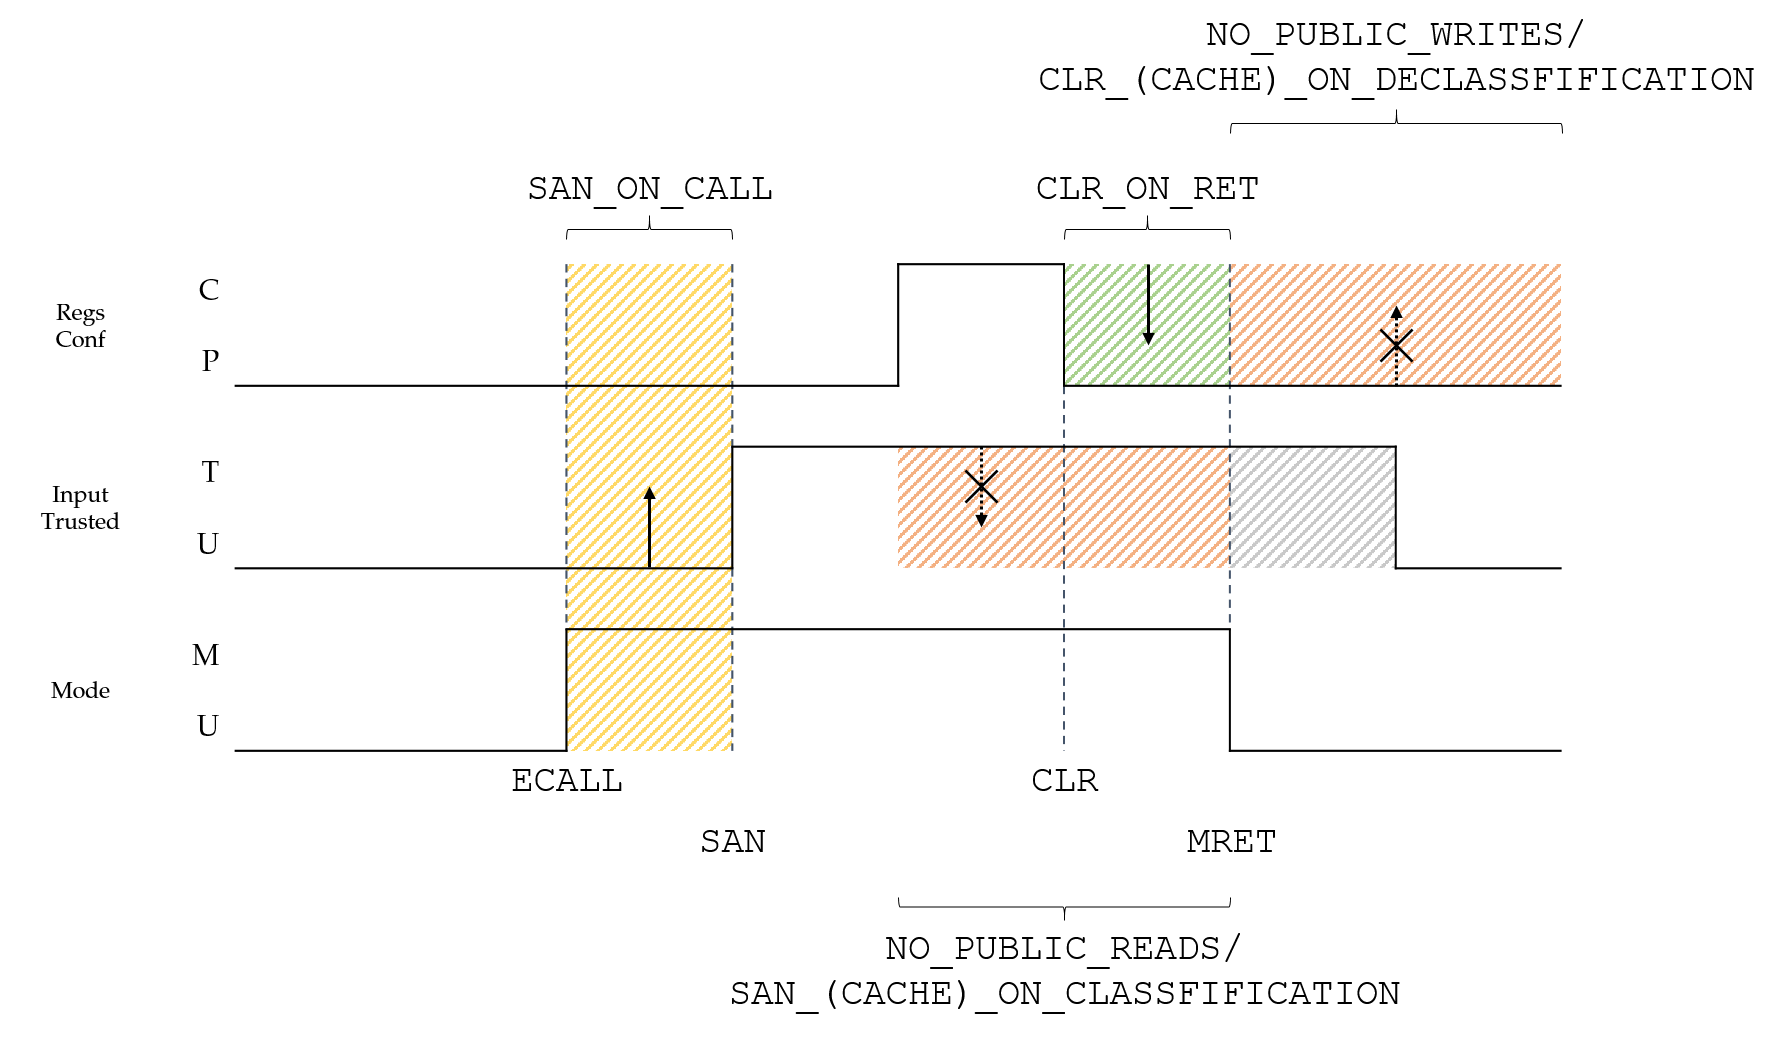
\includegraphics[width=\textwidth]{figures/assumptions.png}
    \caption{Assumptions visualized}
\end{figure}
